\chapter{ Introduction}

\indent MESONH is an atmospheric simulation model which can be run in very different
conditions. Its capabilities are completely described in the scientific
documentation of the model, where the model equations and the whole
physics are given.  

This book gives the  necessary information to perform
numerical experiments, using the MESONH atmospheric system. 
It will help the user to install MESO-NH and to prepare 
a numerical experiment made by this model.\\

From a technical point of view, no special knowledge are required to perform a
simulation. It is useful to specify the main characteristics of
the model: 
\begin{itemize}
\item
The sources are written in {\bf standard Fortran 90} ( Metcalf and Reid 1993)
\item
The source file management is done with {\bf git }
\item
The generalized use of {\bf  dynamic memory allocation} avoids  repeated 
compilation of the source and the free parameters are set by the user
 through namelist files
\end{itemize}

To realize an experiment with MESONH, the user will made a sequence of elementary steps. This sequence will differ according to the type of the simulation : ideal or real, with grid-nesting or not. The different steps  are :

\begin{enumerate}
\item
{\bf PREP\_PGD}: this program computes the physiographic data file.
 At this step, you choose the projection, horizontal resolution
and domain. The PGD file contains all the physiographic data
necessary to run the MESO-NH model with interactive surface schemes for
vegetation and town. PREP\_PGD is presented in chapter \ref{c:PGD}.
\item
{\bf PREP\_NEST\_PGD }: this MESO-NH program checks all the PGD files  to impose
conformity of orography between them. This program is only used with grid-nesting simulations. (see chapter \ref{c:PGD})
\item 
{\bf ZOOM\_PGD }: this program allows to zoom  a PGD file  on the part of interest to make an inner domain at the same resolution. (see chapter \ref{c:PGD})
\item 
{\bf PREP\_IDEAL\_CASE }: this MESO-NH program prepares an initial MESONH file, 
that contains all the parameters and fields necessary for the execution of the model.
 (grid parameters, initial fields and geophysical fields). It is presented in chapter \ref{c:PREPIDEAL}.
\item
{\bf extractecmwf}\footnote{A user account is necessary on the station ecgate of ECMWF to run
{\bf extractecmwf}} 
or {\bf extractarpege}\footnote{A user account at METEO FRANCE is necessary to run
{\bf extractarpege}} 
: it extracts the surface
and altitude fields for a specific date, respectively for ECMWF archive 
(ECMWF forecast model) or
METEO-FRANCE operational archive (ARPEGE, AROME and ALADIN models).
In both cases, the fields are written in a GRIB format file, on the gaussian
grid. The extraction must be done separately for each date and time (for
the initial file and each of the coupling file). The Unix procedures used for these extractions are not presented in this book.
\item 
{\bf PREP\_REAL\_CASE }: this MESO-NH program performs the change of
orography and vertical grid by interpolating horizontally and vertically for a 
GRIB file or only vertically for a MESO-NH file. The MESO-NH output file  will
 be used either for the beginning of the simulation or for coupling. It is presented in chapter \ref{c:PREPREAL}.
\item
{\bf SPAWNING} : this program performs the horizontal interpolations from a
MESO-NH file into another MESO-NH file, with a finer resolution and smaller
domain. (see chapter \ref{c:SPAWNING})
\item
{\bf MESONH } : it is the temporal integration of the model. This step is developped in details in chapter \ref{ch:model}.
\item 
{\bf DIAG } : this program performs diagnostic variables after the simulation. To have more information on this program see chapter \ref{ch:diag}.
\item
{\bf SPECTRE }: this program, presented in chapter \ref{ch:spectre}, performs a particular diagnostic : energy spectra.
\end{enumerate} 

The figures 1.1  and 1.2  present the sequence of the steps for an ideal simulation and a real simulation in mono-model case and with grid-nesting respectively. Detailed sequences for grid-nesting simulation are described in annexe \ref{a:sequence}.
\begin{center}
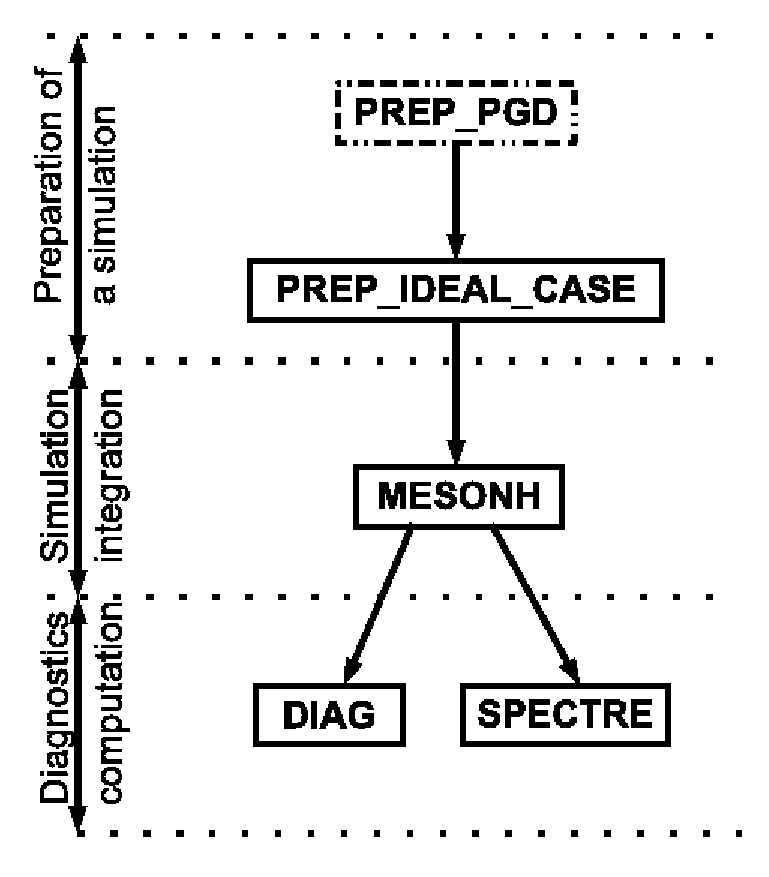
\includegraphics[width=6cm]{intro/magie3}
\\
\textit{Figure 1.1 : General algorithm for an idealized numerical experiment }
\end{center}
\begin{minipage}{8cm}
\vspace{5cm}
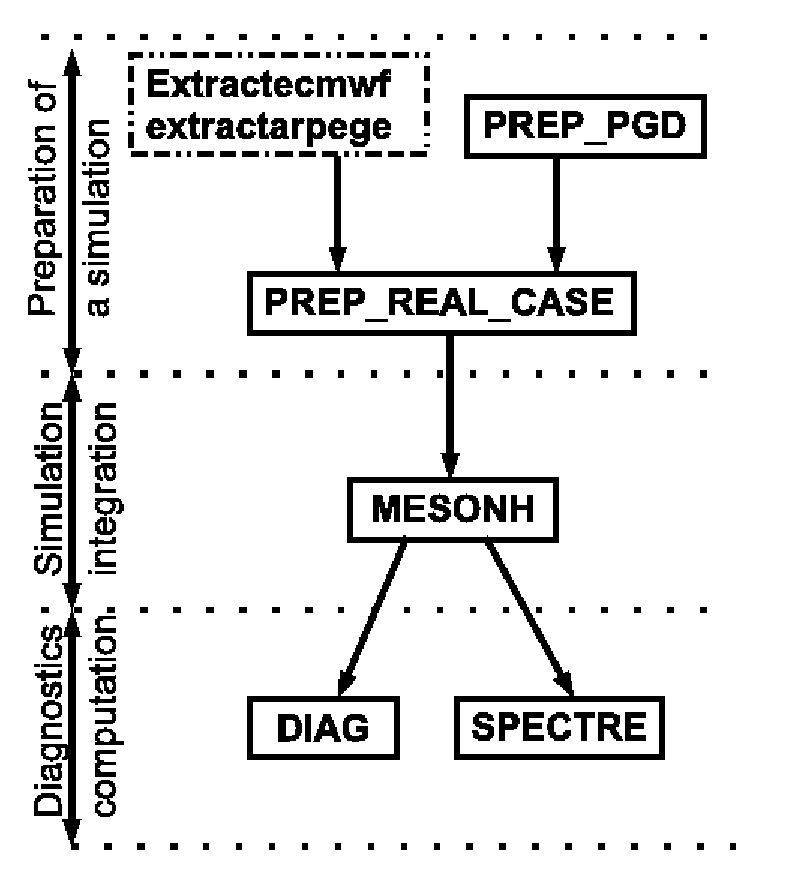
\includegraphics[width=7cm]{intro/magie2}
\begin{center}
\textit{mono-model}
\end{center}
\end{minipage}
\begin{minipage}{9cm}
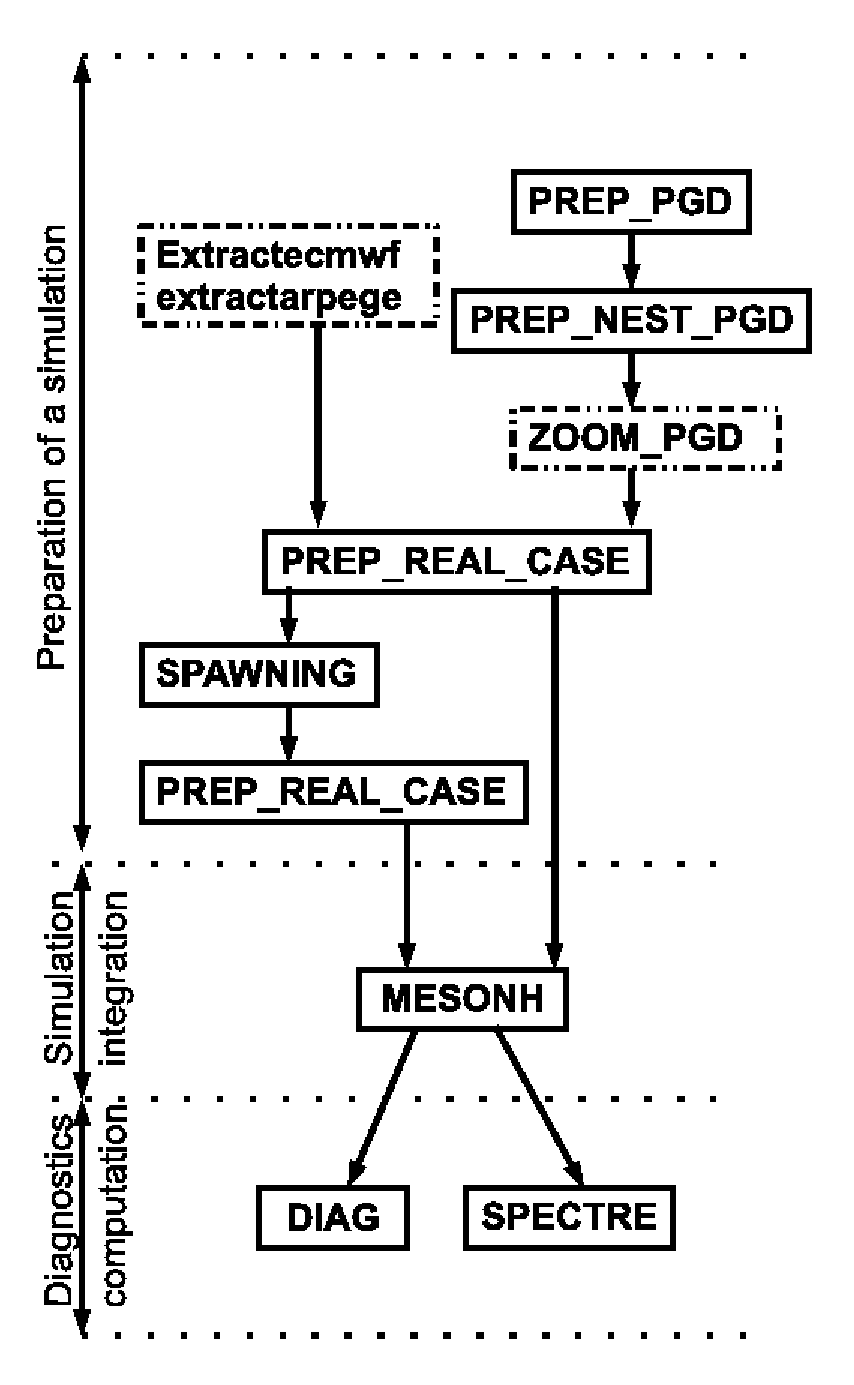
\includegraphics[width=7.5cm]{intro/magie}
\begin{center}
\textit{with grid-nesting}
\end{center}
\end{minipage}
\begin{center}
\textit{Figure 1.2 : General algorithm for a real numerical experiment}
\end{center}




\newpage



First, in chapter 2, we wil present how to install MESONH and how to compile 
personal sources.
Then in chapter 3, the MESONH files (namelists and FM file) are described in details.
In chapter 4 to 11, we will describe every elementary step of MESONH.
In Annexe A,  we will list all the variables present in a FM-file, in annexe B, we will describe sequences for grid-nesting simulation ; in annexe C, we present in details the LES diagnostics. Finally, in annexe D you will find a description of the MESO-NH grid.
 
